\subsection{\textbf{RQ1:} How do developers approach merge conflicts?}\label{RQ1}

To understand the perspective of developers when encountering a merge conflict, we asked interview participants a series of open-ended questions regarding situations, information needs, contributing factors, and processes that are followed when initially evaluating a merge conflict.

The results of our interview indicate that developers recognize certain traits of a merge conflict as contributing to the overall difficulty of the conflict.
Card sorting of interview transcripts resulted in 9 distinct categories that relate to these traits: \textit{Temporal}, \textit{Deadlines}, \textit{Patch Management}, \textit{Atomicity}, \textit{Size of Conflict}, \textit{3-Way Merge Conflicts}, \textit{Code Style}, and \textit{Domain Knowledge} (see Table~\ref{interview_tags}).
These trait categories served as the foundation for the questions and answers included in our survey.

\begin{table}[!]
\renewcommand{\arraystretch}{1.3}
\caption{Merge Conflict Difficulty Categories from Interviews}
\label{interview_tags}
\centering
\begin{tabularx}{0.5\textwidth}{@{}{c}@{ }{c}@{ }p{4.5cm}}
\toprule
	Category & \# Cards & \hfil Description \\
\midrule
	Atomicity & 6 & Consolidation of changes based upon logic units. \\
	Patch Management & 5 & Ordering of patches to prevent merge conflicts. \\
	Code Complexity & 4 & How complex the lines of conflicting code are. \\
	Code Style & 3 & Subtle changes that cause conflicts due to spacing, renaming, etc.\\
	Deadlines & 3 & Increased rates of developer error leading up to deadlines. \\
	Size of Conflict & 3 & Larger commits, or higher volumes of commits, leading to conflicts. \\
	Domain Knowledge & 2 & Awareness about conflicting lines and surrounding code. \\
	Temporal & 1 & Elapsed time between commits in a merge conflict. \\
	3-Way Merge Conflicts & 1 & Multiple commits involved in a single conflict. \\
\bottomrule
\end{tabularx}
\end{table}

We also asked survey participants to rate how much particular factors, derived from the interviews, have an effect on their perceptions of how difficult a merge conflict will be. These factors are observable or estimable traits of the conflict, which means that they are factors that developers can use when initially assessing merge conflicts.
Each factor was ranked in Table \ref{survey_merge_conflicts} based on a 5-point Likert scale consisting of the following answer options:
(1) Not at all (2) A little (3) A moderate amount (4) A lot (5) A great deal.

\begin{table*}[!]
\renewcommand{\arraystretch}{1.3}
\caption{Factors of Merge Conflict Difficulty from Survey}
\label{survey_merge_conflicts}
\centering
%\begin{tabularx}{0.9\textwidth}{@{}r|*{6}{C}c@{}}
\begin{tabularx}{0.78\textwidth}{r | *5{c} | *3{c}}

\toprule
	Factor & 1 & 2 & 3 & 4 & 5 & Mean & Median & Std. Dev. \\
\midrule
	\textbf{Complexity of conflicting lines of code} & 5 & 29 & 38 & 56 & 34 & \textbf{3.52} & 4 & 1.10 \\
	\textbf{Your knowledge/expertise in area of conflicting code} & 5 & 23 & 50 & 54 & 30 & \textbf{3.50} & 4 & 1.05 \\
	Complexity of the files with conflicts & 8 & 34 & 49 & 51 & 18 & 3.23 & 3 & 1.07 \\
	Number of conflicting lines of code & 2 & 40 & 64 & 45 & 11 & 3.14 & 3 & 0.91 \\
	Time to resolve a conflict & 14 & 56 & 51 & 25 & 15 & 2.82 & 3 & 1.09 \\
	Atomicity of changesets in the conflict & 20 & 48 & 51 & 29 & 13 & 2.80 & 3 & 1.12 \\
	Dependencies of conflicting code on other components & 20 & 56 & 39 & 33 & 14 & 2.78 & 3 & 1.16 \\
	Number of files in the conflict & 10 & 69 & 50 & 26 & 6 & 2.68 & 3 & 0.94 \\
	\textbf{Non-functional changes (whitespace, renaming, etc.)} & 47 & 63 & 31 & 15 & 4 & \textbf{2.16} & 2 & 1.03 \\
\bottomrule
\end{tabularx}
\end{table*}

\underline{\textit{Code Complexity:}} Cyclomatic complexity \cite{mccabe1976complexity} is a well-established measure of code complexity in software. However, it has also been criticized as being based on poor theoretical foundations \cite{Shepperd1988}, and not all software developers have experience using it. So for this study, we intentionally left the interpretation of the word ``complexity'' to the individual participants.
In the interview, P4 commented on how the size of the conflict impacts its difficulty, saying,

\begin{displayquote}
\textit{``The size is usually not the issue. Just the complexity of the code that happens to be with the conflicting state.''}	
\end{displayquote}
\todo{Maybe find another participant or two that also motivate this?}
Since P4 did not explicitly state whether he meant complexity of the lines of code in the conflict or complexity of the files in the conflict (which accounts for a bigger-picture view of the code), we asked participants about both line complexity and file complexity. Our results show that both line complexity (mean of 3.52) and file complexity (mean of 3.23) rank above \textit{Number of conflicting lines of code} (mean of 3.14). This suggests that complexity impacts the apparent difficulty of the conflict more than size. However, it is also possible that conflict size is part of what defines conflict complexity, which would mean that size cannot be more impactful than complexity.

\underline{\textit{Domain Knowledge:}} Domain knowledge represents the developer's knowledge of the area of code where the conflict is located. In the interview, P5 said, 

\begin{displayquote}
	\textit{``A lot of what I work on is\textellipsis in my own little area, so when there is a merge conflict in that area, I will know what to do\textellipsis But if I'm\textellipsis in the [other part of project], then I'll\textellipsis get someone else to\textellipsis resolve the merge conflict for me\textellipsis It's someone else's, and I don't want to screw it up.''}
\end{displayquote}

This participant found domain knowledge to be important enough that he would find someone who is familiar with the code around the merge conflict rather than resolving the conflict himself. In the event of non-intuitive code, this option is a helpful approach to resolution because it does not require the developer to fully understand the code before resolving. It also takes into consideration other changes that may be happening around that conflict resolution that would be affected by a bad merge.

%The results of our survey indicate that \textit{complexity of conflicting lines of code} and \textit{knowledge/expertise in the area of conflicting code} are factors that practitioners find have a direct effect on the perceived difficulty of a merge conflict.
%Although we found consensus across all demographics, the experience level of respondents had an affect on the degree to which they responded affirmatively for these factors (see Table~\ref{survey_merge_conflicts}).
%
%Practitioners with 1-5 years and 6-10 years of experience were only nominally in agreement that merge conflict difficulty is affected by \textit{complexity of conflicting lines of code} (mean: 3.31 and mean: 3.37 respectively) and \textit{knowledge/expertise in the area of conflicting code} (mean: 3.21 and mean: 3.42 respectively).
%As practitioner experiences increases, the level of agreement increases on both of these factors, with practitioners indicating 26+ years experience having the highest consensus (mean: 4.06, std. deviation: 0.77). 
%
%Larger, more complex projects typically require that developers have more experience and a higher degree of knowledge about the systems used in the project.
%As the size of a software project increases, so does the complexity of the underlying code~\cite{banker1993software}\cite{curtis1979third}.
%Therefore, more experienced practitioners are likely to have a broader range of understanding about both \textit{complexity of conflicting lines of code} and \textit{knowledge/expertise in the area of conflicting code} and their affects on merge conflict difficulty.
%
%\begin{figure}[!t]
%\centering
%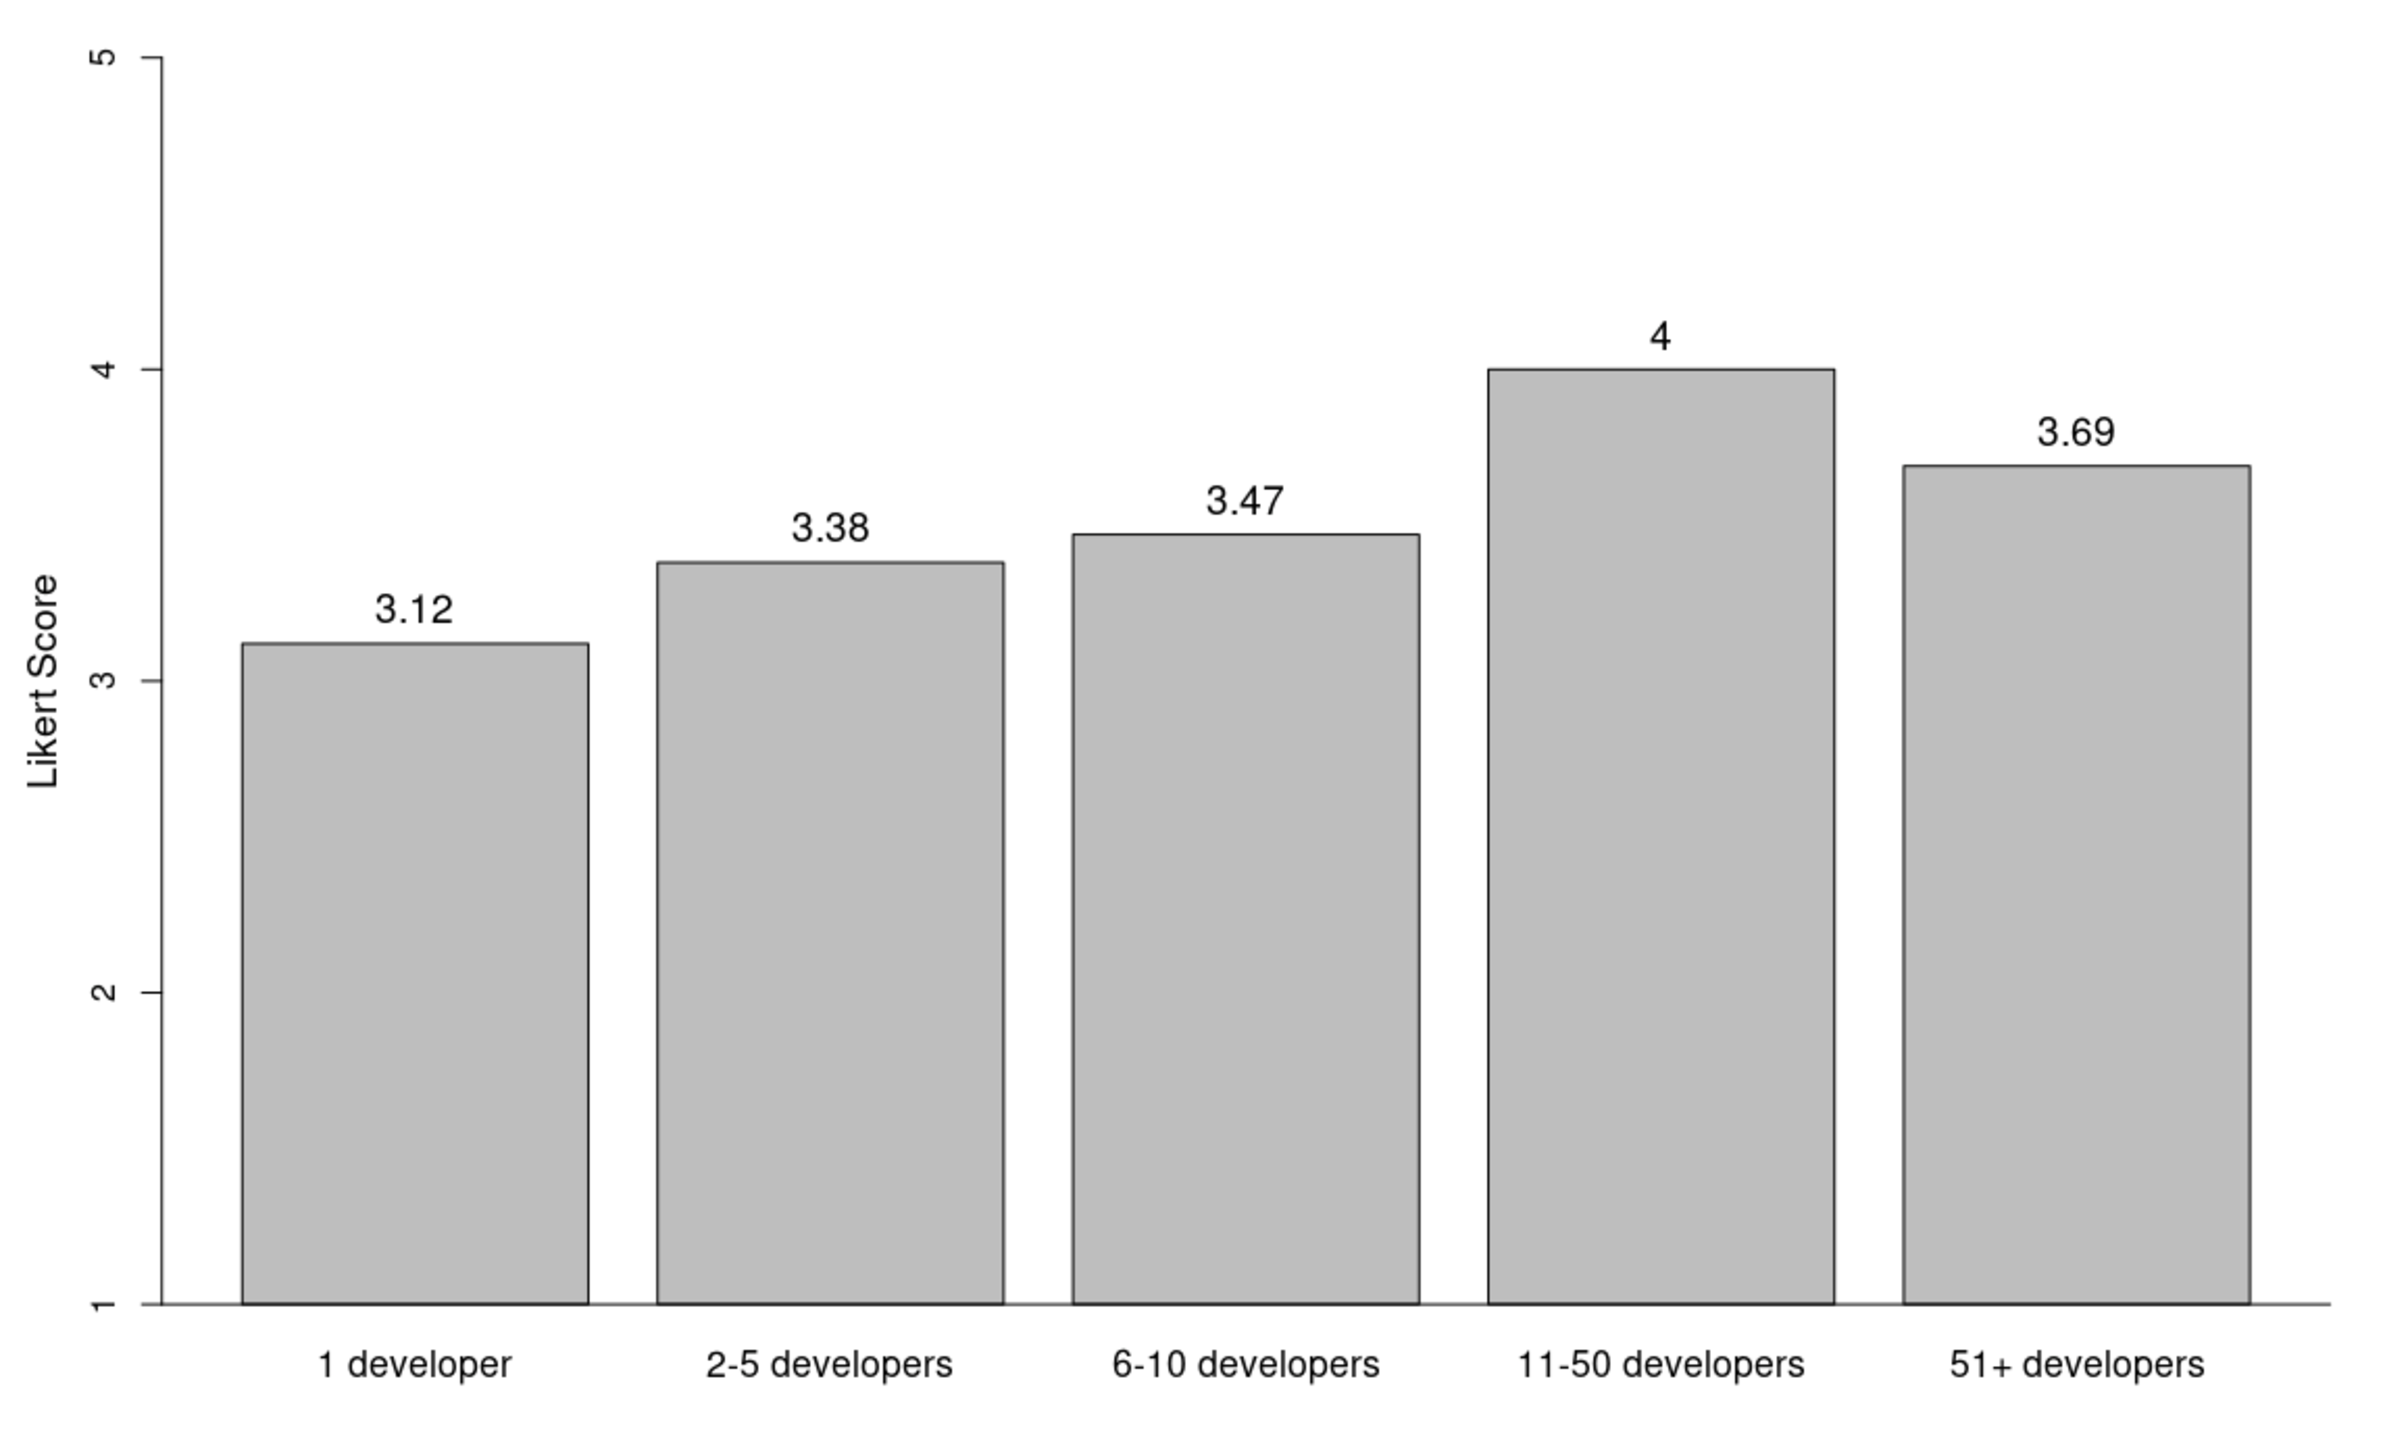
\includegraphics[width=3.4in]{MeanProjectSize.pdf}
%\caption{Mean Likert Score by Project Size for \textit{knowledge/expertise in the area of conflicting code} category of factors that effect the perceived difficulty of merge conflicts.}
%\label{mean_likert_project_size}
%\end{figure}
%
%When analyzing by the size of project that practitioners normally work on, we found that \textit{knowledge/expertise in the area of conflicting code} was increasingly viewed as having an effect on merge conflict difficult as the practitioners' project size increased (see Figure~\ref{mean_likert_project_size}).
%The practitioners that usually work in project sizes of \textit{1 developer}, \textit{2-5 developers}, and \textit{6-10 developers} had relatively neutral responses regarding the effects of \textit{knowledge/expertise in the area of conflicting code} (mean: 3.12, mean: 3.38, and mean: 3.47 respectively).
%However, practitioners that usually work in project sizes of \textit{11-50 developers} and \textit{51+ developers} more positively indicated that \textit{knowledge/expertise in the area of conflicting code} has an effect on the difficulty of merge conflicts (mean: 4.00 and mean: 3.69 respectively).
%
%We also found that practitioners agree that \textit{non-functional changes (whitespace, renaming, etc.)} (mean: 2.16, std. deviation: 1.03) has no effect on the perceived difficulty of a merge conflict.
%Non-functional changes are textual conflicts that can be resolved without consideration of dependencies, performance, or scope.
%Practitioners have less to reason about when resolving merge conflicts that involve only textual conflicts, and therefore are unlikely to perceive \textit{non-functional changes} as affecting the difficulty of merge conflicts.

%Intuitively, we would assume that an increased perception of \textit{knowledge/expertise in the area of conflicting code} as difficulty factor would correlate with a decreased perception of \textit{complexity of conflicting lines of code} as a difficulty factor of merge conflicts.
%This relationship would indicate that a developer's expertise allows them to rationalize about merge conflicts with higher complexity, since they have a higher degree of past knowledge in that area of conflict.
%However, we find a statistical significant correlation between \textit{complexity of conflicting lines of code} and \textit{knowledge/expertise in the area of conflicting code} (Pearson's correlation coefficient: 0.2766, p-value: 0.0003664, 95\% confidence interval: 0.1279 0.4132).
%This suggests that ...

%%%%%%%%%%%%%%%%%%%%%%%%%%%%%%%%%%%%%%%%%%%%%%%%%%%%%%%%%%%%%%%%%

%\subsubsection{Interviews}
%%The interview results suggest that developers approach merge conflicts...
%
%\subsubsection{Survey}
%Our survey suggests that regardless of gender, developer role, experience level, project size, and source distribution model, software practitioners say that the following factors affect the difficulty of a merge conflict most: 
%\begin{itemize}
%\item \textit{Complexity of conflicting lines of code}
%\item \textit{Your knowledge/expertise in area of conflicting code}
%\end{itemize}
%
%Similarly, software practitioners across every measured demographic perceived the following factors to be less important when deciding the difficulty of a merge conflict:
%\begin{itemize}
%\item \textit{Non-functional changes (whitespace, renaming, etc)}
%\item \textit{Number of files in the conflict}
%\end{itemize}
%
%While survey participants did not agree that non-functional changes strongly factor into the difficulty of a merge conflict, it is still worth noting that several interview participants named non-functional changes, such as large refactor or reformatting changes, as a cause for merge conflicts. This suggests that non-functional changes may increase the likelihood of a merge conflict happening, but they do not contribute to the conflict's difficulty.
%
%However, some demographics do view certain difficulties. For instance, open-source developers think that \textit{Atomicity of change sets in the conflict} impacts the difficulty, while closed-source developers and people who split their time evenly think that atomic change sets have no effect on the difficulty. This may be explained by the findings in Rigby et al\cite{OSS_smaller_commits}, which shows that open-source projects tend to review smaller changes than closed-source projects because "The small size lets reviewers focus on the entire change, and the incrementality reduces reviewers’ preparation time and lets them maintain an overall picture of how the change fits into the system." It is possible that our result reflects this difference of culture.
%
%We also found that Project Maintainers say that \textit{Time to resolve a conflict} has an effect, while no other role agrees. This suggests that those in a maintainer role may be more subject to time-related constraints such as maintenance or release schedules. 
%
%\comment{Project Managers say no effect because they focus on project schedules, not conflict resolutions, i.e. they are higher level/abstraction?}
%
%\todo{might be previous work}
%Support and infrastructure roles (System Engineer, Sys Admin, System Architect, DevOps) emphasized that \textit{Dependencies of conflicting code on other components} have more of an effect than other roles did. This might be due to infrastructure systems being maintained in a live environment, or systems that are currently in production use and at risk of real-time dependency failures. 
%
%Developers on projects of size 1 say that \textit{Dependencies of conflicting code on other components}. Because no other project sizes agree with this idea, we hypothesize that this could be due to their high dependence on external code because of the software production limitations of a 1-developer team.
%
%We also found that the group of developers with 21-25 years of experience frequently contradicted general consensus, but it seems more likely that these differences were simply due to the group's small sample size (4).

%We asked participants how much they trust their merging, history exploration, and/or conflict resolution tools, and 57.9\% of participants reported that they trusted these tools either \textit{A Lot} or \textit{Completely}. While this is a majority of developers, this still leaves a significant number of people (42.1\%) who trust their tools \textit{A moderate amount} or \textit{A little}. Though we had the option for \textit{Not at all}, no participants selected this option, presumably because users stop using tools that they do not trust at all. While we found no previous work discussing the threshold for how much users must trust tools for a good tool experience, we postulate that users who cannot trust their tools \textit{A Lot} or \textit{Completely} will avoid relying on such tools too much.